\chapter{Framing Learning Problems}
\label{ch:framing-learning-problems}

Many AI projects begin with an ambition that sounds sensible but is still too vague to support technical work. ``Use AI for student success.'' ``Detect bad content.'' ``Find fake news.'' These are not yet learning problems. They are institutional intentions. If a team begins building from that level of abstraction, it often produces a system whose outputs are mathematically polished but practically confused.

This chapter turns that kind of ambition into a defensible learning problem. The central task is not to choose a model early, but to specify the user, the action, the proxy target, the acceptable inputs, and the evidence that could later justify the claim. By the end of the chapter, the goal is to have a concise \emph{framing memo}: a short statement of the task, the decision context, the inputs, and the standard of evidence that makes later modeling work worth doing.

\section{Problem-Solving Technique: Decision-First Framing}

\begin{problemsolvinglens}
Before choosing a model, ask what decision is being supported, what measurable target can stand in for that decision, what data will make the task visible, what form of the input the model will actually receive, and how the later claim will be judged.
\end{problemsolvinglens}

\begin{thinkingtool}
\textbf{Decision-first framing.} State the action, the constraint, and the cost of mistakes before selecting a candidate model. A model becomes meaningful only inside that decision context.
\end{thinkingtool}

\begin{practicalnote}
A simple workflow is enough to start: write the decision, name the user, choose a proxy target, list acceptable and excluded inputs, and then draft a memo that makes the action and review path, meaning who interprets the output before action, explicit. If that sequence feels fuzzy, the problem is still not ready for model choice.
\end{practicalnote}

\section{Opening Dilemma: A Messy Real Problem}

Suppose a university asks: \emph{Can we identify students who may need help early?} That sounds like a sensible use of AI. It is also not yet precise enough to support technical work, meaning that the goal has not yet been translated into a usable technical specification.

The first weak version of the request is usually something like ``predict weak students.'' That phrase hides nearly every important technical and ethical decision. Who is the user of the system? What action will follow? What counts as ``weak''? Are we predicting missed deadlines, low quiz scores, course failure, or disengagement from the learning platform? Which inputs are acceptable, and which would be inappropriate or unavailable at prediction time? What is the most harmful mistake: missing a student who needs help, or bothering a student who does not?

Already we can see the real educational point. The opening task is not to choose a model. It is to turn an institutional concern into a problem that can be specified, evaluated, and defended.

If the problem statement remains vague at this point, later mathematical sophistication will mostly conceal the confusion rather than resolve it.

Keep one broader institutional setting in view from the start of the book: a course-support organization trying to help students earlier and more reliably. In Chapter 1, that setting appears first as early-outreach risk scoring. Later it will widen into message routing, policy retrieval, grounded answering, and escalation. The workflow changes, but the framing discipline does not.

\begin{practicalnote}
The second running case---a pedestrian detector for a campus shuttle---will appear fully in Chapter~\ref{ch:vision}. It requires the same framing discipline as the course-support assistant: What counts as a pedestrian? At what distance? Under what lighting? The vision-specific constraints are deferred, but the framing questions are identical. Keep this case in mind as a preview of how problem framing generalizes beyond text and tabular data.
\end{practicalnote}

\begin{practicalnote}
Before the chapter develops the full protocol, it is worth seeing what a rough first-pass framing memo already looks like.
\end{practicalnote}

\begin{table}[t]
\centering
\small
\setlength{\tabcolsep}{4pt}
\begin{tabular}{L{3.06cm}L{7.17cm}}
\toprule
Field & Rough first-pass entry for the opening dilemma \\
\midrule
Decision and user & Adviser or instructor decides whether to invite a student to a check-in or tutoring conversation \\
Proxy target & Risk of missing the first two major deadlines or failing to submit early core work rather than a vague idea such as ``weak student'' \\
Acceptable inputs & Early quizzes, assignment submissions, attendance, and learning-platform activity related to the course \\
Costliest mistake & Missing a student who needed timely human support \\
Downstream action & Outreach and support, not punishment or automated judgment \\
Review path & A human adviser interprets the score in context \\
\bottomrule
\end{tabular}
\caption{A rough memo is better than a vague ambition. The chapter will refine this into a fuller framing artifact later, but students should see the target shape early.}
\label{tab:rough-framing-memo}
\end{table}

This table is intentionally incomplete. Its job is only to make the chapter's destination visible early. The fuller framing memo later in the chapter adds excluded inputs, evaluation preview, and cleaner justification for the task. The rest of Chapter 1 can be read as the work needed to justify each row.

The argument develops by making each hidden design choice explicit: first the decision, then the proxy target, then the evidence, and only after that the model.

Once the problem is framed at this level, only a small amount of field orientation is needed. The next step is not a survey of AI as a whole, but a clearer view of where machine learning sits inside that larger landscape and why it is the right focus for the rest of the chapter.

\section{Brief Orientation: Where Machine Learning Fits}

Artificial intelligence is a broad label. It includes search, planning, reasoning, robotics, knowledge representation, and machine learning. In this book we focus mainly on machine learning because it provides the dominant framework for modern AI systems in vision, language, speech, recommendation, forecasting, and many decision-support applications.

This distinction matters only to orient the scope. The chapter's main work is still problem framing rather than field taxonomy.

\begin{figure}[t]
\centering
\definecolor{c1aiBg}{RGB}{235,242,253}
\definecolor{c1mlBg}{RGB}{189,212,240}
\definecolor{c1dlBg}{RGB}{56,103,170}
\definecolor{c1aiLine}{RGB}{56,103,170}
\resizebox{\linewidth}{!}{%
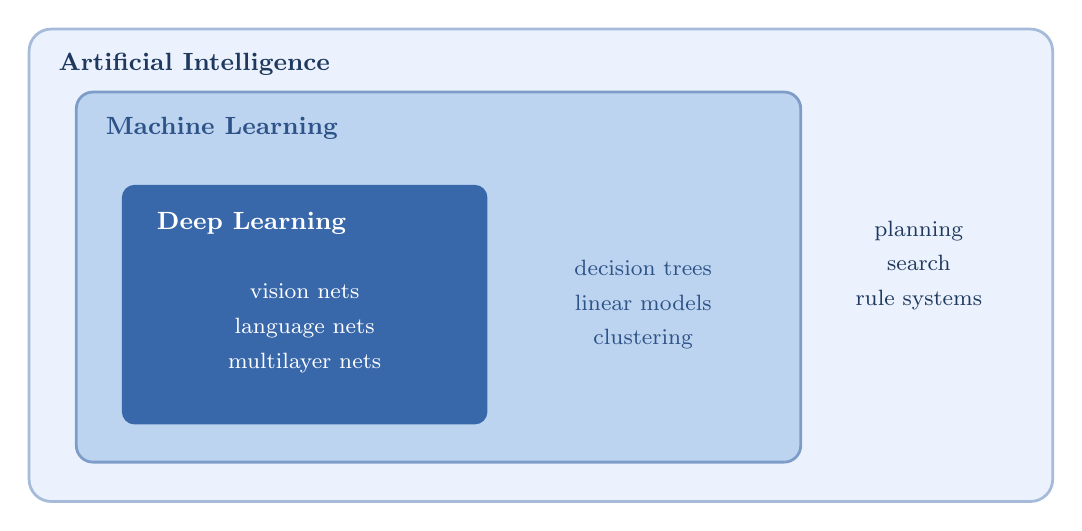
\begin{tikzpicture}[x=1cm, y=1cm, font=\small]
%% ── Outer AI zone ────────────────────────────────────────────────────────
\draw[rounded corners=8pt, fill=c1aiBg, draw=c1aiLine!45, line width=1pt]
    (0,0) rectangle (13.0,6.0);
%% ── Middle ML zone ───────────────────────────────────────────────────────
\draw[rounded corners=6pt, fill=c1mlBg, draw=c1aiLine!65, line width=1pt]
    (0.6,0.5) rectangle (9.8,5.2);
%% ── Inner DL zone ────────────────────────────────────────────────────────
\draw[rounded corners=4pt, fill=c1dlBg, draw=c1aiLine, line width=1.2pt]
    (1.2,1.0) rectangle (5.8,4.0);
%% ── Zone labels ──────────────────────────────────────────────────────────
\node[anchor=north west, font=\small\bfseries, text=c1aiLine!55!black]
    at (0.25,5.82) {Artificial Intelligence};
\node[anchor=north west, font=\small\bfseries, text=c1aiLine!80!black]
    at (0.85,5.0) {Machine Learning};
\node[anchor=north west, font=\small\bfseries, text=white]
    at (1.5,3.8) {Deep Learning};
%% ── DL examples ──────────────────────────────────────────────────────────
\node[align=center, text width=2.6cm, font=\footnotesize, text=white]
    at (3.5,2.2) {vision nets\\[3pt]language nets\\[3pt]multilayer nets};
%% ── ML-only examples ─────────────────────────────────────────────────────
\node[align=center, text width=2.2cm, font=\footnotesize, text=c1aiLine!80!black]
    at (7.8,2.5) {decision trees\\[3pt]linear models\\[3pt]clustering};
%% ── AI-only examples ─────────────────────────────────────────────────────
\node[align=center, text width=2.3cm, font=\footnotesize, text=c1aiLine!55!black]
    at (11.3,3.0) {planning\\[3pt]search\\[3pt]rule systems};
\end{tikzpicture}%
}
\caption{Deep learning is a subset of machine learning, and machine learning is a subset of the broader AI field.}
\label{fig:ai-ml-dl}
\end{figure}

Machine learning is the part of AI concerned with improving performance through data or experience rather than through fully hand-written rules. Sometimes that experience comes with labels, meaning desired outputs attached to examples. Sometimes it comes through rewards, raw data, or targets created from the data itself. The common structure is that we define a set of candidate models and use data to select or adapt one that behaves usefully.

\begin{table}[t]
\centering
\small
\setlength{\tabcolsep}{4pt}
\begin{tabular}{L{2.23cm}L{3.82cm}L{3.9cm}}
\toprule
System style & Where the behavior mostly comes from & Typical Chapter 1 example \\
\midrule
Rule-based system & Hand-written rules, search, or symbolic logic designed in advance & A student-support system that fires fixed alerts when two assignments are missed \\
Machine learning system & A model fitted from examples, often using hand-designed summaries of the input & A spam detector trained on labeled email using counts of which words appear \\
Deep learning system & A multi-layer model that learns internal features from large data rather than relying mostly on hand-designed ones & A neural vision model for counting objects from aerial images \\
\bottomrule
\end{tabular}
\caption{The boundary is not absolute, because real systems often combine learned components with rules and search. The table is meant only to orient the reader before the framing method begins.}
\label{tab:ai-ml-dl-contrast}
\end{table}

It is helpful to introduce a small amount of notation early because it clarifies what is being learned. Suppose each example consists of an input $x$ and a desired output $y$, often called a label. A dataset can be written as
\[
\mathcal{D} = \{(x_1, y_1), (x_2, y_2), \ldots, (x_n, y_n)\}.
\]
The model is a function $f_\theta$ with parameters $\theta$, the adjustable numbers that training will tune, and its prediction for an input $x$ is
\[
\hat{y} = f_\theta(x).
\]

\begin{prereqbridge}
At this stage, read the notation informally: $x$ is the input, $y$ is the desired output, $\theta$ is the adjustable part of the model, and $\hat{y}$ is the model's prediction.
\end{prereqbridge}

That notation is enough for now. Chapter 1 is not about manipulating formulas. It is about deciding what the symbols should refer to in the first place. That small bit of notation is enough to state a central distinction: predicting $\hat{y}$ from $x$ is not the same thing as deciding what to do with $\hat{y}$.

\section{Prediction Is Not the Decision}

The book's first major distinction is simple and easy to forget: a prediction is not the same thing as a decision.

Spam filtering is a clean contrast case. Public resources such as the Enron Corpus and the Apache SpamAssassin project make it concrete rather than fictional \citep{klimt2004,spamassassin}. The model may output a score, for example an estimated probability $P(y=1 \mid x)$, meaning the model's estimated chance that a message is spam given the email $x$. But the product still has to decide what action follows. One cutoff, also called a threshold, may trigger a warning. A higher cutoff may quarantine the message. The same underlying score can therefore support several different policies.

The same distinction returns immediately to the student-support opening. A risk score might trigger an adviser review, a tutoring invitation, or no action at all. Those are different policies built on the same predictive output.

\begin{figure}[t]
\centering
\definecolor{c1zoneg}{RGB}{210,238,220}
\definecolor{c1zonea}{RGB}{254,242,214}
\definecolor{c1zoner}{RGB}{254,216,216}
\resizebox{\linewidth}{!}{%
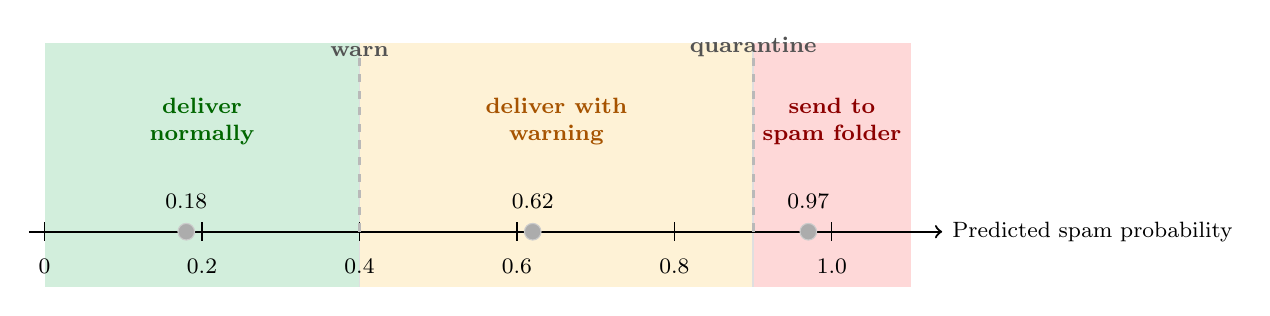
\begin{tikzpicture}[x=1cm, y=1cm, font=\small]
%% ── Colored zone backgrounds ─────────────────────────────────────────────
\fill[c1zoneg] (0,-0.7) rectangle (4,2.4);
\fill[c1zonea] (4,-0.7) rectangle (9,2.4);
\fill[c1zoner] (9,-0.7) rectangle (11,2.4);
%% ── Zone dividers ────────────────────────────────────────────────────────
\draw[gray!25, line width=0.6pt] (4,-0.7) -- (4,2.4);
\draw[gray!25, line width=0.6pt] (9,-0.7) -- (9,2.4);
%% ── Axis ─────────────────────────────────────────────────────────────────
\draw[->, thick] (-0.2,0) -- (11.4,0)
    node[right, font=\footnotesize] {Predicted spam probability};
\foreach \x/\lbl in {0/0, 2/0.2, 4/0.4, 6/0.6, 8/0.8, 10/1.0}
    \draw (\x,0.12) -- (\x,-0.12) node[below=3pt, font=\footnotesize] {\lbl};
%% ── Threshold lines ──────────────────────────────────────────────────────
\draw[dashed, gray!55, line width=1pt] (4,0) -- (4,2.2);
\draw[dashed, gray!55, line width=1pt] (9,0) -- (9,2.2);
\node[above, font=\footnotesize\bfseries, gray!65!black] at (4,2.1) {warn};
\node[above, font=\footnotesize\bfseries, gray!65!black] at (9,2.1) {quarantine};
%% ── Zone action labels ───────────────────────────────────────────────────
\node[align=center, font=\footnotesize\bfseries, text=green!40!black]
    at (2,1.4) {deliver\\normally};
\node[align=center, font=\footnotesize\bfseries, text=orange!65!black]
    at (6.5,1.4) {deliver with\\warning};
\node[align=center, font=\footnotesize\bfseries, text=red!55!black]
    at (10,1.4) {send to\\spam folder};
%% ── Example data points ──────────────────────────────────────────────────
\filldraw[fill=gray!65, draw=gray!40] (1.8,0) circle (3pt)
    node[above=5pt, font=\footnotesize] {$0.18$};
\filldraw[fill=gray!65, draw=gray!40] (6.2,0) circle (3pt)
    node[above=5pt, font=\footnotesize] {$0.62$};
\filldraw[fill=gray!65, draw=gray!40] (9.7,0) circle (3pt)
    node[above=5pt, font=\footnotesize] {$0.97$};
\end{tikzpicture}%
}
\caption{Prediction is not the same as decision. The same model score can feed several product actions through thresholds chosen by humans.}
\label{fig:spam-thresholds}
\end{figure}

When a system marks a legitimate email as spam, that mistake is called a \emph{false positive}. When spam gets through untouched, that mistake is called a \emph{false negative}. Those names matter because the two mistakes usually have different costs.

\begin{table}[t]
\centering
\small
\setlength{\tabcolsep}{4pt}
\begin{tabular}{L{2.25cm}L{3.85cm}L{3.85cm}}
\toprule
Mistake type & What happens & Why the cost matters \\
\midrule
False positive & A legitimate email is treated as spam & The user may miss bills, job offers, travel updates, or personal messages \\
False negative & Spam reaches the inbox & The user faces annoyance, wasted attention, fraud attempts, or malware risk \\
\bottomrule
\end{tabular}
\caption{Prediction quality depends on the consequences of mistakes, not only on whether the model makes an error in the abstract.}
\label{tab:spam-mistakes}
\end{table}

\begin{table}[t]
\centering
\small
\setlength{\tabcolsep}{4pt}
\begin{tabular}{L{1.76cm}L{2.02cm}L{6.16cm}}
\toprule
Student & Risk score & Action at threshold 0.70 \\
\midrule
A & 0.12 & No outreach \\
B & 0.29 & No outreach \\
C & 0.48 & No outreach \\
D & 0.62 & No outreach \\
E & 0.74 & Invite to adviser review \\
F & 0.91 & Invite to adviser review \\
\bottomrule
\end{tabular}
\caption{A score becomes a decision only after a threshold is chosen. The scores stay fixed when the policy changes.}
\label{tab:threshold-worked-example}
\end{table}

If the threshold moved to 0.50, student D would also be reviewed. If it moved to 0.80, only student F would be reviewed. The prediction itself does not change; only the decision rule does.

\begin{mathlens}
\begin{theorem}[Monotone Score Transformations Preserve Ranking]
Let $s(x)$ be a real-valued score and let $g$ be a strictly increasing function. Then for any two cases $x_i$ and $x_j$,
\[
s(x_i) < s(x_j) \iff g(s(x_i)) < g(s(x_j)).
\]
\end{theorem}

\begin{proof}[Proof Sketch]
If $s(x_i) < s(x_j)$ and $g$ is strictly increasing, then applying $g$ preserves the inequality, so $g(s(x_i)) < g(s(x_j))$. The reverse direction follows in the same way because a strictly increasing function cannot reverse the order of two unequal inputs.
\end{proof}

So any ranking based only on score order is unchanged if the score is replaced by a strictly increasing transformation of that score. This is one reason ranking quality and probability calibration should be treated as different questions: a transformed score can preserve the ranking while changing the numerical meaning of the output.
\end{mathlens}

\begin{figure}[t]
\centering
\resizebox{\linewidth}{!}{%
\begin{tikzpicture}[
  box/.style={draw, rounded corners, align=center, minimum height=0.95cm, minimum width=2.1cm, fill=black!4},
  arrow/.style={-Latex, thick}
]
\node[box] (world) {Real-world\\process};
\node[box, right=0.9cm of world] (data) {Collected\\data};
\node[box, right=0.9cm of data] (model) {Chosen model\\$f_\theta$};
\node[box, right=0.9cm of model] (pred) {Prediction\\$\hat{y}$};
\node[box, right=0.9cm of pred] (decision) {Decision\\rule};
\node[box, below=1.2cm of model] (outcome) {Observed\\outcome};
\draw[arrow] (world) -- (data);
\draw[arrow] (data) -- (model);
\draw[arrow] (model) -- (pred);
\draw[arrow] (pred) -- (decision);
\draw[arrow] (decision) |- (outcome);
\draw[arrow] (outcome) -| (data);
\end{tikzpicture}%
}
\caption{A learning problem does not end at the model. Real systems move from world to data to prediction to decision and then back to new outcomes.}
\label{fig:world-to-decision}
\end{figure}

This is why the book begins with framing rather than algorithms. A score without a downstream action is incomplete, and an action without a stated cost of mistakes is hard to defend.

\section{Objective Hierarchy: Goal, Proxy, Label, Metric}

One reason beginner projects drift so quickly is that several levels of description get collapsed into one vague sentence. A team says it wants to ``improve retention'' or ``support students better,'' then jumps directly to labels and metrics as if they were the same thing as the institutional goal. They are not.

Keep four levels separate. The \emph{goal} is the real-world outcome that matters. The \emph{proxy target} is the narrower learning task that stands in for that goal. The \emph{label rule} turns that target into observed examples. The \emph{metric} is the number reported after development. A fifth quantity enters as soon as training begins: the \emph{objective}, the penalty minimized during fitting. In student support, the proxy target might be the risk of missing one of the first two major deadlines or failing to submit early core work; the objective might be log loss on the labeled examples; and the metric might be recall under a fixed review budget. A project can talk about one quantity, optimize another, and report a third, so the names are not interchangeable.

\begin{table}[t]
\centering
{\footnotesize
\setlength{\tabcolsep}{3pt}
\renewcommand{\arraystretch}{1.0}
\begin{tabular}{@{}>{\raggedright\arraybackslash}p{1.38cm}>{\raggedright\arraybackslash}p{2.08cm}>{\raggedright\arraybackslash}p{4.45cm}>{\raggedright\arraybackslash}p{1.90cm}@{}}
\toprule
Level & Core question & Student-support example & Common failure \\
\midrule
Goal & What real-world outcome matters? & Help more students receive timely human support before early disengagement compounds & Treating an institutional hope as if it were already measurable \\
Proxy target & What narrower learning task stands in for that goal? & Predict risk of missing the first two major deadlines or failing to submit early core work early enough to intervene & Choosing a proxy that is easy to log but poorly aligned with the real need \\
Label & How will the proxy be turned into observed targets? & Mark a case positive if the student misses one of the first two major deadlines or fails to submit early core work by the review cutoff & Treating administratively produced labels as ground truth rather than as measurements \\
Metric & What number will summarize success? & Recall among students who trigger the early-support proxy event, measured under a fixed advising-review budget & Optim\-izing a convenient number that ignores the decision constraint \\
\bottomrule
\end{tabular}
\caption{Keep goal, proxy target, label construction, and reporting metric separate rather than pretending they are all the same thing.}
}
\label{tab:objective-hierarchy}
\end{table}

The difference becomes clearer in one concrete student-support story. The institutional goal is not ``predict failure'' in the abstract. The goal is to help students receive timely human support. The proxy target might therefore be the risk of missing the first two major deadlines or failing to submit early core work, because waiting for final-course failure would make the intervention too late. The label then depends on a measurable rule that records whether one of those early-support events occurred by the review cutoff. The reported metric may finally be recall at a fixed review budget because the advising team can inspect only a limited number of cases each week.

Notice what happened. The project became more precise at every step, but it also became more honest about where mismatch can enter. A weak project often fails not because the model is poor, but because these four levels were never separated cleanly enough to inspect.

\begin{thinkingtool}
\textbf{Objective hierarchy.} Before writing code, write four short sentences: the real-world goal, the proxy target, the label rule, and the reporting metric. If two of the sentences sound identical, the problem is probably still underframed.
\end{thinkingtool}

\section{The Five Commitments}

Many beginner mistakes come from starting with a favorite model rather than with the structure of the problem. A more reliable approach is to identify five commitments before training begins and to answer them in order.

\begin{enumerate}[leftmargin=*,label=\arabic*.]
\item \textbf{Task.} What exactly is the system supposed to predict, estimate, rank, or decide?
\item \textbf{Data.} What evidence will stand in for the world?
\item \textbf{Representation.} What form of the input will the model actually see?
\item \textbf{Objective.} What behavior is rewarded during training?
\item \textbf{Evaluation.} What later claim will count as success?
\end{enumerate}

Read these commitments as operational checkpoints rather than as vocabulary words. Each one makes the next one more concrete. Task says what must be learned. Data and representation make that task visible. Objective says what training will reward. Evaluation states what later evidence must support.

These five commitments are Chapter 1's local framing protocol inside the book's broader seven-question framework. They explain how a vague request becomes a learnable task before baseline, reliability, and systems questions are added later.

The book's broader seven-question framework can be stated compactly:
\begin{enumerate}[leftmargin=*,label=\arabic*.]
\item What decision or action is being supported?
\item What target will stand in for that decision?
\item What evidence about the world is actually available?
\item What representation will the model really see?
\item What baseline must be beaten?
\item What evidence would justify the claim?
\item What system will carry the prediction into action?
\end{enumerate}

The Five Commitments are a local workshop version of that larger framework. Task mainly answers Questions 1 and 2. Data answers Question 3. Representation answers Question 4. Evaluation previews Question 6. Questions 5 and 7 are delayed because a framing chapter should first make the problem legible before it asks what baseline is credible or what deployment system will be responsible for the output. Objective is added here because once a task is framed, training still needs a concrete signal about what the model should learn to do.

This is also the right place to connect the two organizing frameworks already introduced. The objective hierarchy from the previous section asks for goal, proxy target, label rule, and reporting metric. The Five Commitments widen that picture: goal and proxy target shape the task, the label rule constrains data collection, representation says what the model actually receives, objective says what training rewards, and evaluation asks what later claim the evidence can support. The hierarchy separates levels of meaning; the commitments turn those levels into a full project frame.

\begin{table}[t]
\centering
\footnotesize
\setlength{\tabcolsep}{2.5pt}
\begin{tabular}{@{}>{\raggedright\arraybackslash}p{2.45cm}>{\raggedright\arraybackslash}p{1.42cm}>{\raggedright\arraybackslash}p{1.72cm}>{\raggedright\arraybackslash}p{1.68cm}>{\raggedright\arraybackslash}p{2.53cm}@{}}
\toprule
Commitment & Guiding question & Student support & Spam filtering & Counting task \\
\midrule
Task & What must be predicted? & Risk of missing the first two major deadlines or failing to submit early core work & Probability an email is spam & Animal count from an aerial image \\
Data & What evidence stands in for the world? & Quizzes, attendance, logs & Labeled email text and message details & Images paired with local count targets \\
Representation & What form does the model actually see? & Early-course signals in a student table & Words, links, sender cues, and email metadata & Pixels, local patches, and count cues \\
Objective & What behavior is rewarded in training? & Minimize a supervised loss that raises scores on students likely to trigger the early-support proxy event in time for human review & Minimize a training loss that separates spam from wanted mail & Minimize error between predicted and observed local count targets \\
Evaluation & What claim is being tested? & Does it support advising without unfair profiling or useless alarms? & Does it protect inboxes without hiding wanted mail? & Does it perform well on evaluation images whose answers stayed hidden during development? \\
\bottomrule
\end{tabular}
\caption{A framing canvas turns the five commitments into concrete questions before model choice begins.}
\label{tab:chapter1-framing-cases}
\end{table}

\begin{practicalnote}
Table~\ref{tab:chapter1-framing-cases} expands the rough memo from Table~\ref{tab:rough-framing-memo} into the chapter's first reusable protocol. If you cannot fill it out clearly, the project is usually not ready for model development.
\end{practicalnote}

The order of use matters. First write the task in operational terms. Then ask what data and representation would make that task visible. Only after that should the training objective and later evaluation claim be written down. In the broader seven-question framework, this table mainly settles Questions 1 through 4 and previews Question 6.

\section{Proxy Audit: From Vague Goal to Defensible Task}

The next move is to repair vague openings. This is the chapter's most reusable habit. A proxy audit forces us to separate the real-world goal from the measurable target we can actually train on. That measurable target is called a \emph{proxy target} because it stands in for the broader goal rather than matching it perfectly.

\begin{thinkingtool}
\textbf{Proxy audit.} Write down the real-world goal and the label you can actually measure. Then list how sampling, timing, annotation, or historical process could make the measured target diverge from the real goal.
\end{thinkingtool}

\begin{table}[t]
\centering
\small
\setlength{\tabcolsep}{4pt}
\begin{tabular}{L{2.83cm}L{7.4cm}}
\toprule
Weak opening & Better framed learning problem \\
\midrule
``Use AI to support students'' & Predict which students are likely to miss the first two major deadlines early enough to trigger human support. \\
``Detect bad content'' & Estimate the probability that a comment should be queued for moderator review under a documented moderation policy. \\
``Find fake news'' & Classify whether an article is likely to violate a specific fact-checking standard, with human review before public action. \\
\bottomrule
\end{tabular}
\caption{The main improvement is not sophistication. It is moving from slogans to tasks with users, targets, and downstream actions.}
\label{tab:bad-to-better-framing}
\end{table}

\begin{decisionbox}
\textbf{Proxy stress test.} Is the proxy measurable, timely, available at prediction time, action-relevant, and hard to game? If any answer is no, revise the proxy before training.
\end{decisionbox}

Notice what changes in each rewrite. The user becomes clearer. The proxy target becomes narrower. The downstream action becomes more defensible. The model has not improved yet. The \emph{problem statement} has.

Once the proxy target is defensible, the next question is whether the available data actually makes that target visible.

\section{What Data Actually Represents}

Students often say that ``the data speaks for itself.'' It does not. Data is produced by instruments, institutions, interfaces, and human choices. A medical image depends on scanner settings and clinical workflow. A text corpus depends on which languages, websites, or books were collected. A recommendation dataset depends on what users were previously shown. A dataset is never the world itself. It is a measurement process applied to the world.

This matters for at least three reasons. First, sampling matters. If the data covers only some users or conditions, the model may generalize poorly elsewhere. Second, labeling matters. If labels are noisy, inconsistent, or based on weak proxies, the model may learn the proxy instead of the intended target. Third, timing matters. Data gathered in one year or one market may not represent the next.

\begin{example}[Recommendation Logs Reflect Exposure]
Recommendation data is a useful warning because the labels are entangled with the system that produced them. A movie platform only observes clicks and ratings for items users were actually shown. AutoDebias describes this as a combination of selection bias and exposure bias: observed ratings are not a representative sample of all possible ratings, and a missing interaction may mean non-exposure rather than dislike \citep{autodebias2021}. That is why a recommender dataset is not a neutral reading of user preference. It is a record of preference filtered through previous ranking decisions.
\end{example}

\begin{example}[Toxicity Labels Are Social Measurements]
Content moderation provides a different kind of warning. Sap et al.\ show that annotator identities and beliefs can systematically affect toxicity judgments \citep{sap2022}. Disagreement is not always random noise that disappears if we average enough labels. Sometimes it reflects real differences in how people interpret harm, offense, and context. A model trained on such labels is therefore learning a socially situated target, not an uncontested ground truth.
\end{example}

\begin{failurebox}
A student-risk model can look strong if one of its inputs is a support flag created only after the first missed deadline. That feature may be predictive, but it is not available at prediction time; it leaks a later process back into the model. The same mistake appears in moderation if a post-hoc moderator outcome is reused as a feature.
\end{failurebox}

For these reasons, it is better to think of a dataset as evidence rather than truth. Evidence can be strong or weak, representative or narrow, stable or outdated. The quality of the learning problem depends on the quality of that evidence.

\begin{practicalnote}
When a new dataset appears, ask three simple questions before trusting it: who or what is missing, how were the labels or measurements produced, and when was the data collected relative to the task you care about?
\end{practicalnote}

\section{Data-Centric ML: Improve the Evidence, Not Only the Model}

Once a task has been framed, beginners often assume that the next improvement must come from a more sophisticated model. In many projects, the faster and more defensible improvement comes from the data instead: clearer label definitions, fewer duplicates, broader coverage, cleaner measurements, or better documentation. Data-centric machine learning means treating data design, collection, annotation, and maintenance as first-class engineering work rather than as a fixed backdrop.

This does not mean ``more data'' in the abstract. It means better evidence for the task actually being asked. If annotators disagree often, the question is not only who made the mistake. The real issue may be that the task definition is ambiguous, that important context was hidden, or that the label space is too coarse for the problem. In that situation, changing the model may help less than changing the data specification.

Documentation matters for the same reason. Gebru et al.\ argue that datasets should come with structured documentation about motivation, composition, collection process, and recommended uses \citep{gebru2018datasheets}. If a team cannot answer basic questions about who was included, how labels were produced, what preprocessing was applied, and which uses are out of scope, then later claims about model quality become difficult to interpret.

In high-stakes settings, weak data practice compounds downstream. Sambasivan et al.\ call these failures \emph{data cascades}: upstream problems in collection, labeling, or coordination can reappear later as model failure, monitoring surprises, or unsafe deployment behavior \citep{sambasivan2021}. A stronger architecture does not automatically repair a weak dataset. It may instead fit the dataset's accidental structure more efficiently.

\begin{thinkingtool}
\textbf{Data iteration loop.} Before replacing the model, inspect failures and ask whether the problem is coverage, label definition, annotation consistency, preprocessing, or version control. Then change one data-side element deliberately and record a new dataset version.
\end{thinkingtool}

Versioning is the practical habit that makes data-centric work scientific rather than anecdotal. If a team removes duplicates, relabels borderline cases, adds examples from an underrepresented setting, or changes preprocessing, then the dataset has changed. The result should be treated as a new version with its own documentation. Chapter~\ref{ch:experiments-claims} returns to this experimental discipline, but the habit starts here, while the problem is still being framed.

\begin{practicalnote}
When a model fails on a recurring slice, do not ask only ``which model should we try next?'' Ask whether the slice is underrepresented, mislabeled, poorly defined, or missing key context. In many real projects, the first serious improvement is a better labeling guide and a versioned dataset release rather than a deeper network.
\end{practicalnote}

Improving the evidence naturally leads to the next issue: how later chapters will decide whether the resulting claim survives new data.

\section{Evaluation Preview: Unseen Data and Hidden Targets}

Chapters 2 and 3 are the real judgment chapters, so evaluation appears here only as a preview. The essential preview is simple: a learning problem is not defined only by its inputs and targets. It is also defined by what counts as unseen evidence. That is why the framing memo already needs an evaluation preview. If you do not know what evidence will stay protected until the end, you do not yet know what claim the project is trying to defend.

In practice, this is why machine learning separates training, validation, and test roles. Some data is used to fit the model. Some may be used to compare settings. Some must remain protected until the end so the reported result means something. Chapter 3 turns that principle into a full evaluation workflow.

The same discipline appears in public benchmark tasks, where some data is released for development and some answers are kept hidden until judging. One useful supporting example is aerial wildlife counting. The input is an aerial image. The output is a density map, meaning a grid of small values spread across the image so that adding them gives the final animal count. The visible data lets the student build a model, but the real claim is judged on hidden targets.

At Chapter 1 level, the detailed metrics can wait. The habit cannot. The habit is to protect some evidence so the final claim is judged on data that development did not already see.

\begin{figure}[t]
\centering
\definecolor{c1visBg}{RGB}{220,233,251}
\definecolor{c1hidBg}{RGB}{228,228,228}
\definecolor{c1modBg}{RGB}{237,224,250}
\resizebox{\linewidth}{!}{%
\begin{tikzpicture}[
  x=1cm, y=1cm, font=\small,
  visbox/.style={draw=blue!40, rounded corners=4pt, align=center,
                 minimum height=1.2cm, minimum width=3.2cm,
                 fill=c1visBg, line width=0.8pt},
  hidbox/.style={draw=gray!50, rounded corners=4pt, align=center,
                 minimum height=1.2cm, minimum width=3.2cm,
                 fill=c1hidBg, line width=0.8pt},
  modbox/.style={draw=purple!38, rounded corners=4pt, align=center,
                 minimum height=1.2cm, minimum width=3.2cm,
                 fill=c1modBg, line width=0.8pt},
  arrow/.style={-Latex, thick, gray!70!black}
]
%% ── Region labels ────────────────────────────────────────────────────────
\node[font=\scriptsize\bfseries, blue!45!black]  at (0, 3.65) {VISIBLE};
\node[font=\scriptsize\bfseries, gray!55!black]  at (7.0, 3.65) {HIDDEN};
%% ── Divider between visible and hidden regions ───────────────────────────
\draw[dashed, gray!40, line width=0.8pt] (2.55,3.85) -- (2.55,-0.35);
%% ── Top row: data splits ─────────────────────────────────────────────────
\node[visbox] (train) at (0,   2.6) {Visible training set\\images + density maps};
\node[hidbox] (valid) at (5.0, 2.6) {Hidden evaluation set\\counts not shown};
\node[hidbox] (test)  at (9.6, 2.6) {Final hidden test set\\counts not shown};
%% ── Model node ───────────────────────────────────────────────────────────
\node[modbox] (model) at (0,   0.4) {Model development\\on visible data only};
%% ── Arrows ───────────────────────────────────────────────────────────────
%% train → model (straight down)
\draw[arrow] (train.south) -- node[right, font=\scriptsize, text=blue!40!black]{trains on} (model.north);
%% model → evaluation set: straight right, then straight up
\draw[arrow, gray!70!black, thick] ([yshift=0.12cm]model.east) -- (5.0,0.52);
\draw[-Latex, gray!70!black, thick] (5.0,0.52) -- (valid.south);
\node[font=\scriptsize, text=gray!55!black, right] at (5.1, 1.4) {evaluate};
%% model → final test set: straight right, then straight up
\draw[arrow, gray!70!black, thick] ([yshift=-0.12cm]model.east) -- (9.6,0.28);
\draw[-Latex, gray!70!black, thick] (9.6,0.28) -- (test.south);
\node[font=\scriptsize, text=gray!55!black, right] at (9.7, 1.4) {final test};
\end{tikzpicture}%
}
\caption{The logic of hidden evaluation is the same as sound machine learning practice: develop on visible data, then judge the claim on targets that were not available during development.}
\label{fig:hidden-evaluation-example}
\end{figure}

\begin{example}[Why the Counting Example Fits Chapter 1]
Aerial wildlife counting is not just a vision task. It is a framing task. The input is clear, but the target is richer than a single class label because it involves a spatial density map and a derived count. The evaluation is fixed in advance and hidden during development. This makes it a clean way to teach that a learning problem is defined by its structure, not only by its architecture.
\end{example}

\begin{evidencebox}
Zech et al.\ studied pneumonia detection from chest radiographs and found that performance changed substantially across hospital systems; the model could rely on hospital-specific cues that were not actually signs of disease \citep{zech2018}. The Chapter 1 lesson is simple: a model can look strong on familiar data and still fail when the measurement process shifts.
\end{evidencebox}

\section{A Bad Framing Memo Rewritten}

Before reading the strong memo, it helps to see the weak version that many real projects begin with.

\begin{table}[t]
\centering
\small
\setlength{\tabcolsep}{4pt}
\begin{tabular}{L{3.08cm}L{7.15cm}}
\toprule
Memo field & A weak student-support memo \\
\midrule
Decision and user & ``Use AI to predict which students will fail'' \\
Proxy target & ``Course failure'' with no time window or intervention logic \\
Acceptable inputs & ``All available student data'' \\
Excluded or sensitive inputs & not stated \\
Most costly mistake & not stated \\
Evaluation preview & ``High accuracy'' \\
Downstream action & ``Intervene'' \\
Review path & not stated \\
\bottomrule
\end{tabular}
\caption{A bad memo is useful because it shows where vagueness hides. The fields are present, but they do not yet support a defensible learning problem.}
\label{tab:bad-framing-memo}
\end{table}

This memo is weak in several different ways. The decision is unclear because no user or workflow is named. The proxy target is late and blunt: by the time final failure is observed, it may be too late to help. The input policy is dangerous because ``all available data'' quietly invites irrelevant or sensitive variables. The evaluation plan is weak because accuracy alone says nothing about review burden, intervention usefulness, or unfair alerts. The downstream action is also underdefined. ``Intervene'' could mean an email, an adviser call, a tutoring offer, or a punitive step, and those actions demand different standards of evidence.

The repair is not to make the memo longer for its own sake. The repair is to make each field operational. Replace ``predict failure'' with an earlier support target. Replace ``all available data'' with course-related signals that exist before the decision moment and that the workflow can justify. Replace ``accuracy'' with an evaluation preview tied to human review and useful intervention. Replace vague action with a stated review path and a bounded support response. Each repaired field should force a later design choice rather than merely sounding more polished.

\begin{decisionbox}
If a framing memo sounds impressive but leaves the user, action, time horizon, sensitive-input boundary, and most costly mistake unclear, the project is not yet ready for model choice. Rewrite the memo before writing the model code.
\end{decisionbox}

The next table is therefore not just a more polished version of the same idea. It is a different kind of object: one that could actually guide data choice, evaluation, and system design.

\section{Worked Framing Memo: Student Support}

Public datasets make this example more than a classroom invention. The Open University Learning Analytics Dataset (OULAD) contains demographic information, assessment data, and virtual-learning-environment interactions across several university courses \citep{kuzilek2017}. Policy work on predictive analytics in higher education makes the institutional side equally clear: early-alert systems can support advising, but they also raise concerns about profiling, opacity, and privacy if they are treated as automated judgments rather than support tools \citep{newamerica2016}.

The system here is a triage tool: it surfaces cases for human support, but it does not explain why a student is struggling and it does not make the final judgment about the student.

Now return to the opening dilemma. A university does \emph{not} want an automated system that decides who will pass or fail. It wants a tool that helps identify students who may benefit from timely human support. Once that shift is made, the framing memo becomes much clearer.

\begin{table}[t]
\centering
\small
\setlength{\tabcolsep}{4pt}
\begin{tabular}{L{3.15cm}L{7.08cm}}
\toprule
Memo field & One defensible student-support entry \\
\midrule
Seven-question focus & Questions 1--4 are written directly here; question 6 appears as an evaluation preview, and question 7 appears through downstream action and review path \\
Decision and user & An adviser or instructor decides whether to invite a student to a check-in, tutoring session, or office-hour conversation \\
Proxy target & Risk of missing the first two major deadlines or failing to submit early core work \\
Representation & One student per row, encoded with early-course features such as quizzes, submissions, attendance, and platform activity \\
Acceptable inputs & Early quizzes, assignment submissions, attendance, and learning-platform activity directly related to the course \\
Available at prediction time & Only early-course signals collected before the support decision; no later grades, no post-deadline outcomes, and no flags created after outreach \\
Excluded or sensitive inputs & Sensitive personal attributes, disability information, or private data unrelated to learning support \\
Training objective & Minimize a supervised loss that raises scores on students likely to trigger the early-support proxy event in time for human review \\
Most costly mistake & Failing to flag a student who needed timely human help \\
Evaluation preview & Later evidence should show that the system surfaces useful cases without creating unfair or noisy alerts \\
Downstream action & Outreach, tutoring offers, office-hour invitations, or scheduling support rather than punishment \\
Review path & An instructor, adviser, or student-support professional interprets the output in context \\
\bottomrule
\end{tabular}
\caption{A framing memo turns a vague request into a concrete learning problem before any model training begins.}
\label{tab:framing-memo}
\end{table}

This is the test for Chapter 1. If the reader can take a messy idea and produce a memo like Table~\ref{tab:framing-memo}, the chapter has done its real job. Everything earlier in the chapter should cash out into this document. In Chapter 2, the evaluation preview inside the memo will become explicit metrics, action rules, and probability checks.

\section{Framing Is Iterative, Not One-Shot}

Students sometimes read a memo like Table~\ref{tab:framing-memo} and assume framing happens once, before the ``real'' modeling work begins. Real projects are usually messier. The first memo is a disciplined starting point, not a sacred object that survives every later piece of evidence unchanged.

Suppose the advising team trains an early model and sees three surprises: many flagged students recover quickly without any support action, so the proxy target may be too noisy; one subgroup is systematically under-flagged because early platform activity is a weak signal for their course format; and the current threshold would send far more students to review than the advising team can actually contact.

None of these findings means the framing work was wasted. They mean the framing must now be revised with evidence rather than defended out of pride.

\begin{table}[t]
\centering
\small
\setlength{\tabcolsep}{4pt}
\begin{tabular}{L{2.62cm}L{2.99cm}L{4.34cm}}
\toprule
Memo field & What early evidence revealed & How the framing should change \\
\midrule
Proxy target & the current early-support proxy was too coarse and mixed routine recovery with serious disengagement & refine the proxy toward repeated non-submission or combine it with review notes \\
Inputs & one course format produced weak platform signals & add course-format awareness or restrict the claim to settings where the inputs are meaningful \\
Downstream action & current threshold overloads the advising queue & rewrite the policy around fixed review capacity or ranking under budget \\
Evaluation preview & aggregate score hid subgroup undercoverage & require slice checks and workload-aware evaluation before any deployment claim \\
\bottomrule
\end{tabular}
\caption{A framing memo should tighten when the first experiments expose mismatch. Revision is not a failure of framing; it is the point of framing under evidence.}
\label{tab:framing-iteration}
\end{table}

This is the more mature habit. Framing begins before model training, but it does not end there. If early experiments expose label noise, unrealistic inputs, missing slices, or impossible review load, the right response is often to rewrite the memo rather than to keep optimizing the original task definition.

\begin{decisionbox}
Treat the first framing memo as version 1, not as final truth. When the first experiments reveal a mismatch between proxy, data, action, and capacity, revise the memo before escalating model complexity.
\end{decisionbox}

\section{Brief Orientation: Learning Settings as Kinds of Feedback}

The chapter's main deliverable is now on the page, so only brief orientation remains. With the framing memo in place, the main learning settings become easier to distinguish by the kind of feedback they provide. In supervised learning, the signal comes from explicit labels. In unsupervised learning, there are no target labels and the task is to organize or summarize structure in the data itself. In self-supervised learning, targets are created from the data so that useful representations can still be learned when manual labels are scarce. In reinforcement learning, feedback arrives through rewards attached to actions over time rather than through correct answers supplied in advance.

\begin{figure}[t]
\centering
\definecolor{c1supBg}{RGB}{212,238,220}
\definecolor{c1unsupBg}{RGB}{254,242,214}
\definecolor{c1selfBg}{RGB}{220,233,251}
\definecolor{c1rlBg}{RGB}{237,224,250}
\resizebox{\linewidth}{!}{%
\begin{tikzpicture}[
  x=1cm, y=1cm, font=\small,
  parbox/.style={draw, rounded corners=4pt, align=center,
                 minimum height=1.25cm, minimum width=2.8cm, line width=0.9pt},
  arrow/.style={-Latex, thick, gray!55}
]
%% ── Four paradigm boxes ──────────────────────────────────────────────────
\node[parbox, fill=c1supBg,   draw=green!40!black]  (sup)   at (0,   1.6)
    {\textbf{\textcolor{green!40!black}{Supervised}}\\[2pt]explicit labels};
\node[parbox, fill=c1unsupBg, draw=orange!55!black] (unsup) at (3.6, 1.6)
    {\textbf{\textcolor{orange!55!black}{Unsupervised}}\\[2pt]no labels};
\node[parbox, fill=c1selfBg,  draw=blue!45!black]   (self)  at (7.2, 1.6)
    {\textbf{\textcolor{blue!45!black}{Self-supervised}}\\[2pt]generated targets};
\node[parbox, fill=c1rlBg,    draw=purple!45!black] (rl)    at (10.8,1.6)
    {\textbf{\textcolor{purple!45!black}{Reinforcement}}\\[2pt]delayed reward};
%% ── Connecting arrows ────────────────────────────────────────────────────
\draw[arrow] (sup.east)   -- (unsup.west);
\draw[arrow] (unsup.east) -- (self.west);
\draw[arrow] (self.east)  -- (rl.west);
%% ── Example text below each box ──────────────────────────────────────────
\node[align=center, text width=2.8cm, font=\footnotesize,
      text=green!38!black]    at (0,   0.35) {student-risk\\prediction};
\node[align=center, text width=2.8cm, font=\footnotesize,
      text=orange!60!black]   at (3.6, 0.35) {student-behavior\\clustering};
\node[align=center, text width=2.8cm, font=\footnotesize,
      text=blue!55!black]     at (7.2, 0.35) {fill-in-the-\\missing-word};
\node[align=center, text width=2.8cm, font=\footnotesize,
      text=purple!55!black]   at (10.8,0.35) {games or tutoring\\actions over time};
\end{tikzpicture}%
}
\caption{Learning settings differ mainly in the kind of feedback they provide. The distinction matters later when model families and data regimes become more specific.}
\label{fig:feedback-spectrum}
\end{figure}

This orientation matters because later modeling choices depend heavily on what kind of feedback is available, how expensive it is, and how directly it answers the task we care about.

If that distinction still feels abstract, keep one sentence only: the kind of feedback available constrains what the system can honestly learn.

\subsection{Reinforcement Learning: A Different Feedback Regime}

In reinforcement learning, the system learns by taking actions and receiving scalar feedback --- a reward --- from the environment. In the online form of RL, there is no fixed dataset of (input, correct-output) pairs; the agent must discover which actions lead to good outcomes through repeated interaction. The agent observes a state, selects an action, observes the resulting new state and a scalar reward, and uses that signal to adjust future behavior. The loop repeats many times, with no human supplying a correct answer at each step. Later chapters also revisit offline RL, where the learner works from historical interaction logs rather than live experience.

\begin{figure}[t]
\centering
\definecolor{c1agentBg}{RGB}{220,233,251}
\definecolor{c1agentLine}{RGB}{56,103,170}
\definecolor{c1actionBg}{RGB}{254,237,215}
\definecolor{c1actionLine}{RGB}{184,92,16}
\definecolor{c1envBg}{RGB}{212,238,222}
\definecolor{c1envLine}{RGB}{26,112,64}
\definecolor{c1rewardBg}{RGB}{237,224,250}
\definecolor{c1rewardLine}{RGB}{92,32,135}
\resizebox{\linewidth}{!}{%
\begin{tikzpicture}[
  x=1cm, y=1cm, font=\small,
  agentbox/.style={draw=c1agentLine, rounded corners=4pt, align=center,
                   minimum height=1.0cm, minimum width=3.0cm,
                   fill=c1agentBg, line width=1.2pt},
  actionbox/.style={draw=c1actionLine, rounded corners=4pt, align=center,
                    minimum height=1.0cm, minimum width=3.0cm,
                    fill=c1actionBg, line width=1.2pt},
  envbox/.style={draw=c1envLine, rounded corners=4pt, align=center,
                 minimum height=1.0cm, minimum width=3.0cm,
                 fill=c1envBg, line width=1.2pt},
  rewardbox/.style={draw=c1rewardLine, rounded corners=4pt, align=center,
                    minimum height=1.0cm, minimum width=3.0cm,
                    fill=c1rewardBg, line width=1.2pt},
  arrow/.style={-Latex, thick}
]
%% ── Clockwise rectangle: Agent (TL) → Action (TR) → Env (BR) → Reward (BL) ─
\node[agentbox]  (agent)  at (0,   1.6) {\textbf{Agent}};
\node[actionbox] (action) at (6.0, 1.6) {\textbf{Action}};
\node[envbox]    (env)    at (6.0, 0  ) {\textbf{Environment}};
\node[rewardbox] (reward) at (0,   0  ) {\textbf{Reward}\,/\,\textbf{New State}};

\draw[arrow, c1agentLine]  (agent.east)   -- node[above, font=\small] {selects}     (action.west);
\draw[arrow, c1actionLine] (action.south) -- node[right, font=\small] {applied to}  (env.north);
\draw[arrow, c1envLine]    (env.west)     -- node[below, font=\small] {returns}     (reward.east);
\draw[arrow, c1rewardLine] (reward.north) -- node[left,  font=\small] {received by} (agent.south);
\end{tikzpicture}%
}
\caption{In reinforcement learning, the feedback signal is a scalar reward earned by taking actions, not a correct label provided in advance. The agent must discover which actions are valuable through repeated interaction.}
\label{fig:rl-preview-loop}
\end{figure}

\begin{table}[t]
\centering
\small
\setlength{\tabcolsep}{3pt}
\small
\begin{tabular}{L{3.00cm}L{3.55cm}L{3.36cm}}
\toprule
Feedback regime & Source of the learning signal & When it applies \\
\midrule
Supervised learning & Correct labels provided by humans or other processes & When labeled examples are available and the task is well-defined \\
Unsupervised learning & Structure in the data itself & When labels are absent and the goal is to discover clusters, low-dimensional views, or other latent structure \\
Self-supervised learning & Targets generated from the data itself & When labels are scarce but the goal is to learn reusable representations from raw data \\
Reinforcement learning & Scalar rewards from environmental interaction & When the system must learn through trial and error rather than from fixed labeled examples \\
\bottomrule
\end{tabular}
\caption{The four main feedback regimes differ in where the learning signal comes from and in the kind of task they suit best.}
\label{tab:feedback-regimes}
\end{table}

\begin{practicalnote}
This book's center of gravity is supervised and self-supervised machine learning. Reinforcement learning appears here only for orientation. Students who want to go deeper should know that RL is the framework behind game-playing agents, robotic control, and some preference-alignment stages of modern language model training. In this book, only that last connection appears later in the language chapter. Reinforcement learning from human feedback (RLHF) has become central to aligning large language models with human preferences, making RL relevant even in settings that begin as supervised learning problems.
\end{practicalnote}

\section{Common Mistakes in First Machine Learning Projects}

Several mistakes appear so often in first machine-learning projects that they are worth naming directly. The most common is starting with a preferred model rather than with the task, the data, the cost of mistakes, and the evaluation plan. Another is treating labels as if they were perfect truth rather than noisy measurements produced by a process. A third is forgetting that a prediction matters only inside a decision workflow, so the user and downstream action remain unspecified. Finally, students often slip from prediction to explanation too quickly, reading predictive features as if they were causal mechanisms when they may only be proxies or shortcuts.

\section{Looking Ahead}

Chapter 1 identifies the task worth modeling. Chapter 2 asks what kind of predictive behavior would actually count as success for that task. Chapter 3 then asks whether the evidence for that judgment can survive protected evaluation on new data. In other words, Chapter 1 writes the claim in operational form; Chapters 2 and 3 test whether later evidence deserves to support it.

\section*{Chapter Summary}

Chapter 1 argues that the first task in machine learning is not model selection but problem specification. A vague institutional aim becomes a defensible learning problem only after prediction is separated from decision, the real-world goal is distinguished from the proxy target and label rule, and the available dataset is treated as evidence rather than truth. The Five Commitments provide a practical local protocol for naming the task, the evidence, the representation, the training objective, and the evaluation preview. The chapter ends with a framing memo because the real achievement at this stage is not a trained model but a question stated clearly enough that later modeling work can answer it honestly.

\begin{studyquestions}
\item Why is ``predict weak students'' a poor opening statement for an AI project?
\item What is the difference between a prediction and a decision?
\item Why are the Five Commitments better understood as Chapter 1's local protocol inside the broader seven-question framework rather than as a list of vocabulary words?
\item In what sense is a dataset evidence rather than truth?
\item What kinds of project improvements count as data-centric rather than model-centric?
\item Why does a hidden-evaluation task such as aerial wildlife counting belong in Chapter 1 even though the full evaluation chapter comes later?
\end{studyquestions}

\begin{exercises}
\item Prediction or decision? For each scenario, say whether it describes a prediction, a decision, or both: a spam score of $0.91$, automatically quarantining an email, estimating whether a student will miss a deadline, inviting a student to office hours, and ranking comments by toxicity risk for a moderator.
\item Rewrite each vague opening into a more defensible task: ``predict weak students,'' ``detect bad content,'' and ``find fake news.'' For each, name a likely user, proxy target, and downstream action.
\item Explain why the same spam-probability model could support different actions at different thresholds without the model itself changing.
\item Give one example each of supervised, unsupervised, self-supervised, and reinforcement learning, but explain them as different feedback regimes rather than as isolated categories.
\item Consider a university dataset containing attendance, quiz scores, and assignment submissions. List three ways in which the data collection process might bias the resulting model.
\item A moderation dataset shows frequent annotator disagreement on sarcasm and reclaimed slurs. Propose one data-centric intervention and explain why it may help more than simply swapping in a larger model.
\item Suppose a moderation model predicts whether an online comment should be flagged for review. Explain why the predicted probability and the final moderation decision should be treated as separate components.
\item Write down a dataset $\mathcal{D} = \{(x_i, y_i)\}_{i=1}^n$ for a problem of your choice. State what $x_i$, $y_i$, $f_\theta$, and $\hat{y}_i$ mean in that context.
\item Use Table~\ref{tab:framing-memo} to write a one-page framing memo for either student support, spam filtering, or a problem from your own field. If you carry one running case through the book, keep this memo and use the same case again in Chapter 2 when you add metrics and action policy.
\end{exercises}

\begin{challengeexercises}
\item Take a problem from your own domain and argue for two different proxy targets. Explain which one you would choose first and what failure mode the rejected proxy invites.
\item Design a counting task analogous to aerial wildlife counting for another domain. State the input, target, representation, objective, and what an evaluation with hidden answers would need to protect.
\item Give an example of a predictive feature that could be useful for a model but unacceptable in deployment. Explain why the framing memo should reject it before training begins.
\item Write a short critique of a published or public AI system description by identifying which part of the framing memo is missing, underdefined, or ethically unstable.
\end{challengeexercises}
